\chapter[SCP-047 微生物诱变剂]{
    SCP-047 Microbial Mutagen\\
    SCP-047 微生物诱变剂
}

\label{chap:SCP-047}

\begin{figure}[H]
    \centering
    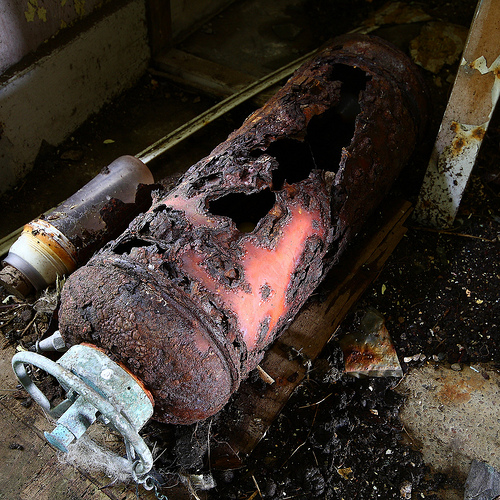
\includegraphics[width=0.5\linewidth]{images/SCP.047.jpg}
    \caption*{收容突破后从Site-██安全实验室回收前位于原位的SCP-047。}
\end{figure}

\bb{项目编号:}SCP-047

\bb{项目分类:}Keter

\bb{特殊收容措施:}SCP-047应被一直收容于一个0.5m x 0.5m x 1m的气密储藏箱中。该箱应被锁入生物安全防护三级实验室047b内的储物柜047a。任何进入047b的行为和室内活动将由生物识别扫描、闭路摄像机和{[}编辑]记录。

进入047b需要该项目主管的批准和至少一个O5级许可。SCP-047在包括接触后的强制隔离在内的所有方案中均应被视为4级传染性生物灾害。为此已在实验室047b配套提供套装q047。

在SCP-047-1的外界污染事件中,必须启动封锁方案047-01“耶尔森氏菌\footnote{\bb{译注:}这种细菌之所以出名是由于其中一种名为“鼠疫耶尔森氏菌”的成员,它能导致黑死病。}”。

\bb{描述:}SCP-047是一个严重锈蚀、破损的储气罐,以铁{[}编辑]合金制成。当被暴露在露天环境下时,该储气罐的材料将缓慢挥发,产生一种之前未被记载的致突变性气体。这种气体对真核生物(例如人类)没有影响,但是会极大地改变原核生物,特别是常见的人体微生物群——在皮肤表面和身体各处自然生存的微生物。少数情况下这种变异产生出一种“超级病菌”(总称为SCP-047-1),即生存能力被增强并因此产生机会性致病性的自然共生微生物。SCP-047引发的变化模式表明这些高传染性的微生物,至少在某种程度上,是经过挑选的。

虽然各种SCP-047-1的具体特性取决于作为其来源的细菌,但有几个特点在所有SCP-047-1变异实例中大体一致:

\begin{itemize}
\item 在该细菌的自然生长环境和其它相似环境下的增强的生存能力;
\item 对所有抗生素的耐药性;
\item 繁殖速度和对可利用原料的消耗加快;
\item 革兰氏阳性菌\footnote{\bb{译注:}革兰氏染色:用来鉴别细菌的一种方法,由丹麦医生汉斯·克里斯蒂安·革兰于1884年发明。革兰氏染色的对象是细菌的细胞壁。不同的细菌在该染色法的作用下反应不同,可分为两类:革兰氏阳性菌,细胞壁染色后呈蓝紫色;革兰氏阴性菌,染色后呈红色。这是辨别细菌种类的重要方法,对由细菌感染引起的疾病的临床诊断及治疗很有帮助。}发展出生成孢子的能力;
\item 增强的吸收、保存和分享质粒\footnote{\bb{译注:}质粒:附加到细胞中的非细胞的染色体或核区DNA原有的能够自主复制的较小的DNA分子。它存在于许多细菌以及酵母菌等生物中,乃至于植物的线粒体等细胞器中。简单来说可以理解为细菌的“遗传物质”。}的能力,尤见于革兰氏阴性菌;
\item 由于上述特点而扩大的传播。
\end{itemize}

SCP-047已选择性地诱变了数种细菌。单独培养的细菌是可能突变的,但该过程对于生存在人类宿主身上的细菌效果显著得多。一般地,鼓励用于实验需要的对自然共生微生物的诱变。在30\slash 01\slash 2010的收容突破之后(参见\hyperref[chap:]{事件报告耶尔森氏菌-047-01(2010)}),对原本就是病原体的种类的诱变被禁止,所有存在的样品都必须销毁。

三种SCP-047-1诱变的特定种细菌由于参与了██\slash ██\slash 201█的收容突破而引起关注:

\tred{+ 展开图片资料}

\tred{- 隐藏图片资料}

\begin{figure}[H]
    \centering
    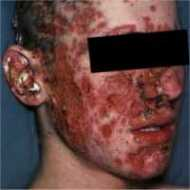
\includegraphics[width=0.2\linewidth]{images/SCP.047.2.jpg}
    \caption*{感染\ii{P-047-A}的D-15978,初次接触2天后。}
\end{figure}

\bb{丙酸杆菌047-A(P-047-A)}是一种由SCP-047诱变的痤疮丙酸杆菌。

\tred{+ 显示详情}

\tred{- 隐藏详情}

\begin{itemize}
\item \bb{致病性:}在皮脂腺周围的皮肤上猛烈增殖。皮肤pH值被调整到对皮肤细胞有毒的程度。极其严重的炎症和免疫细胞的渗漏。皮肤结构的最终崩溃导致败血症。
\item \bb{传播:}皮肤接触传播。能够在无机物表面保持最长五小时活性。
\item \bb{致命性:}死亡率约40\%。病情发展时间2-6周。(感染后)5-10小时内出现非常明显的症状;2-5小时内开始有传染性。
\item \bb{处理:}出现可见症状的受害者必须立即隔离。死亡的受害者应被火化。
\end{itemize}

\bb{链球菌047-C(S-047-C)}是一种由SCP-047诱变的缓症链球菌。

\tred{+ 显示详情}

\tred{- 隐藏详情}

\begin{itemize}
\item \bb{致病性:}最初引起口腔和食道炎症。导致口腔开放性溃疡,使S-047-C进入血液循环感染其它部位。死因通常是感染性内心膜炎。
\item \bb{传播:}有些类似气溶胶;不通过呼吸传播,但偶尔通过咳嗽和吐痰传播。能通过孢子来无限期保持活性。
\item \bb{致命性:}约35\%死亡率。若不致命则可能成为反复发作的慢性疾病。
\item \bb{处理:}有任何口腔感染迹象的对象应被隔离。死亡的受害者应被火化。
\end{itemize}

\bb{梭状芽孢杆菌047-A(C-047-A)}是一种由SCP-047诱变的艰难梭状芽孢杆菌。

\tred{+ 显示详情}

\tred{- 隐藏详情}

\begin{itemize}
\item \bb{致病性:}未知。C-047-A由组织培养法得到,从未被暴露给人类。没有现存于基金会控制下的样品。
\item \bb{传播:}未知。可能和艰难梭状芽孢杆菌一样通过粪便污染传播。由于其更小、更坚固的孢子,可能也和肠胃胀气⑤混合成气溶胶。吸收C-047-A气溶胶的效果无法预测。
\item \bb{致病性:}未知。假设有破坏胃肠道内皮的极高风险,导致发炎、败血症、中毒性巨结肠。
\item \bb{处理:}在进一步研究完成之前,受害者应被隔离并置于全天候医疗观察之下以研究该品种的机能诊断学。死亡的受害者不应在完成足够的病原学研究前被火化。
\end{itemize}

\bb{回收记录047:}SCP-047于██\slash ██\slash 199█由一支基金会生物灾害恢复小队在对一次完全破坏状况的响应中从Site-██安全实验室回收。测试日志表明研究团队当时正试图将{[}数据删除]收容在一个██级抗SCP压缩储气罐中,导致{[}编辑]与{[}编辑]混合。对此的全面分子生物学分析可在{[}编辑]找到。SCP-047结构被破坏时气体的首次释放引发了一次种类不计其数的SCP-047-1的“过量繁殖”,在█小时内杀死了实验室内的所有员工。被沾染的Site-██员工遵从了标准基金会隔离\slash 收容方案,感染被成功收容。
